% !TEX root = ../FinalReport.tex
\chapter{User Guide --- GTM Agent}\label{user-guide-gtm-agent}

\section{What is GTM Agent?}\label{what-is-gtm-agent}

Winning work on big public construction, infrastructure and IT projects starts
with finding the right opportunities, but the EU publishes thousands of new
tenders every week, in dozens of languages. GTM Agent does that reading for you. It follows
the EU's official tenders service (TED), picks out the ones that fit your business and,
for each one, shows you the companies most worth approaching, explains \emph{why} in
plain words, and even writes a first outreach email you can edit and send.

In short: \textbf{GTM Agent turns thousands of public tenders into a short,
ready-to-act list of sales leads, each with a draft email attached.} You can work
through the steps yourself, or just tell the built-in assistant what you want.

\textbf{60-second pitch video:} \url{https://photos.app.goo.gl/fG1kagP8WnbJAEF17}

\section{Who is it for?}\label{who-is-it-for}

\begin{table}[H]
\centering
\caption[Target user groups]{Target user groups and what GTM Agent does for
each.}\label{tab:users}
\begin{tabularx}{\textwidth}{@{}lX@{}}
\toprule
\textbf{Role} & \textbf{What GTM Agent does for them} \\
\midrule
\textbf{Sales / business-development} (primary) & Finds live tenders in their
field, shows which companies to approach, and hands over ready-to-send outreach
emails. \\
\textbf{Buyer / contracting authority} (secondary) & Gets a short list of the
strongest suppliers for a tender. \\
\textbf{Power user} & Runs the whole thing just by describing the goal in plain
words. \\
\bottomrule
\end{tabularx}
\end{table}

\section{How it works}\label{how-it-works}

Five steps take you from a tender to a ready-to-send email, or you can hand the whole
thing to the built-in agent:

\begin{center}
\begin{tikzpicture}[>=Stealth, node distance=5mm]
  \node[flowbox] (s1) {Browse\\tenders};
  \node[flowbox, right=of s1] (s2) {Open \&\\run matcher};
  \node[flowbox, right=of s2] (s3) {Review ranked\\companies};
  \node[flowbox, right=of s3] (s4) {Generate\\email};
  \node[flowbox, right=of s4] (s5) {Rate\\\faThumbsUp\ /\ \faThumbsDown};
  \foreach \a/\b in {s1/s2, s2/s3, s3/s4, s4/s5}{\draw[->] (\a) -- (\b);}
  \draw[->, dashed] (s5.south) to[out=-90, in=-90]
       node[midway, below, font=\scriptsize] {learns from your feedback} (s3.south);
\end{tikzpicture}
\end{center}

Browse tenders in your sectors, open one to run the matcher, review the ranked
companies (each with an explainable score), generate an outreach email or a buyer
digest, then rate the result 👍 / 👎, and the system learns from your feedback.

\textbf{Agent mode (shortcut):} prefer to just \emph{say what you want}? The built-in
agent does steps 1--4 from a single sentence and asks you to confirm if anything is
ambiguous.

\section{Features}\label{features}

\subsection{Find the right tenders}\label{tender-discovery}

The \textbf{Tenders} screen lists live EU opportunities in your field, filtered by
CPV code (the EU's standard procurement categories), each showing the buyer,
country, budget and deadline. Open any one to see its full
details, including a link back to the original public notice, so you can always
check the source for yourself (Figure~\ref{fig:tenders}).

\screenshot[The Tenders screen]{Tendors-tab.png}{Browse live EU tenders on the left;
open one for the full details on the right.\label{fig:tenders}}

\subsection{See who to approach, and why}\label{lead-matching}

Open a tender and GTM Agent instantly lists the companies most likely to win it,
drawn from everyone who has won a comparable EU contract in the award history it has
already collected. It
never hands you a mystery score: for every company you can see how well it fits on
four simple measures: the kind of work it does, the procurement category it fits
(its CPV code), its typical budget, and where it's based, plus a
short note on what mattered most. You always know why a name is on the list (Figure~\ref{fig:matches}).

\subsection{Tune the ranking to your judgement}\label{adjustable-weighting}

Know something the data doesn't, say, that a company is too small for this job?
Drag a slider to give location or budget more importance, and the list re-orders as
you watch. Happy with the result? Click \textbf{Apply} and GTM Agent remembers your
preference for that tender, so it's still there when you come back.

\screenshot[The Matches screen]{Matching-tab(weights).png}{The Matches screen: ranked companies with a
clear breakdown of why each one fits, plus sliders to re-order the list by what
matters most to you.\label{fig:matches}}

\subsection{Send an email that's ready to go}\label{email-generation}

Pick a company and GTM Agent writes a tailored outreach email for you. It only ever
uses real, checkable facts, the tender's reference and deadline, and the company's
own track record. It even writes in the tender's own
language: a French tender gets a French email. Nothing is ever sent automatically;
the draft is yours to review, edit and send. You can also produce a short digest for
a buyer, recommending the strongest suppliers for their tender (Figure~\ref{fig:email}).

\subsection{Rate a result, and it gets better}\label{feedback}

A quick thumbs-up 👍 or thumbs-down 👎 on any match or email tells GTM Agent what a
good lead looks like to your team. The more you use it, the more its suggestions lean
toward the kind of leads you actually want.

\screenshot[A generated email draft]{Emails-tab.png}{A ready-to-send draft, written
only from real facts and in the tender's own language.\label{fig:email}}

\begin{figure}[htbp]
\centering
% Placed with the email figure so both land on one page; equal height lines them up.
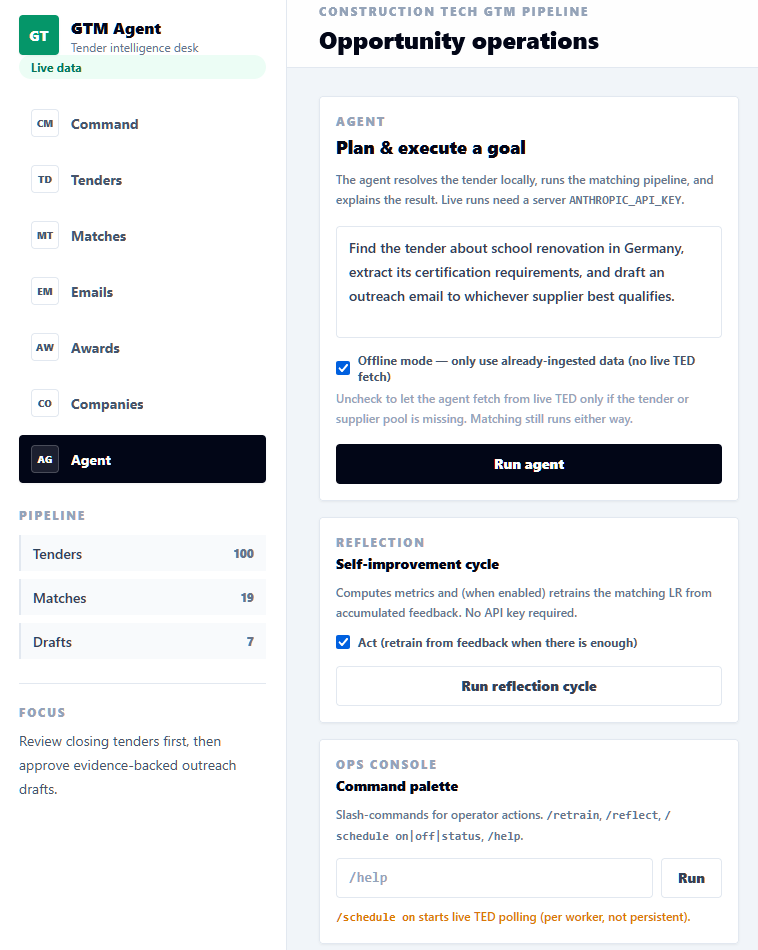
\includegraphics[height=8.5cm]{Agent-mode.png}\hspace{3mm}%
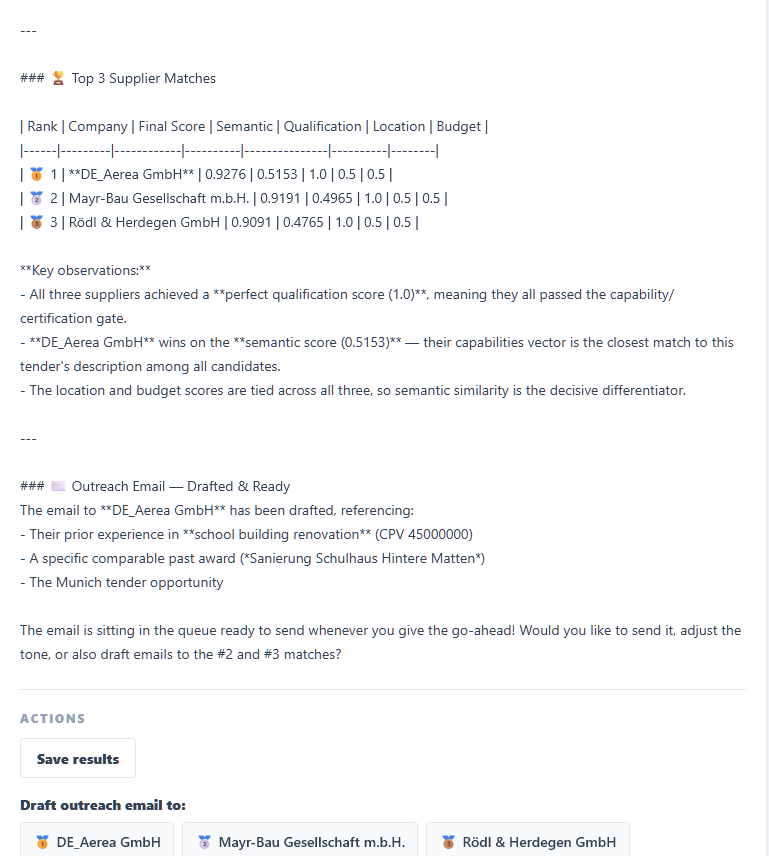
\includegraphics[height=8.5cm]{Agent-mode(Summary-EmailDraft).png}
\caption[Agent mode]{Ask in plain words: the assistant runs the steps live (left) and returns a ranked result (right).\label{fig:agent}}
\end{figure}

\subsection{Agent mode for power users: Just say what you want}\label{agent-mode}

Prefer not to click around? Tell the built-in assistant, in plain words,
for example, \emph{``Find the tender about school renovation in Germany, extract its certification requirements, and draft an outreach email to whichever supplier best qualifies.''} It works through the steps for you and shows what it's doing as it
goes (Figure~\ref{fig:agent}). A few things make it easy to trust:

\begin{itemize}
\tightlist
\item
  \textbf{Name a tender any way you like}, by its title or its official TED notice
  number (for example 420398-2026). If several could match, it stops and asks you
  to pick one instead of guessing.
\item
  \textbf{It stays on your data.} An ``Offline mode'' toggle is on by default, so it
  only uses the tenders and companies already loaded and won't reach out to the internet.
\item
  \textbf{One-click follow-ups.} When it's done, \textbf{save the result} or
  \textbf{draft an email} to any of the top matches in a single click.
\end{itemize}


\section{A typical session (walkthrough)}\label{a-typical-session}

\begin{enumerate}
\def\labelenumi{\arabic{enumi}.}
\tightlist
\item
  Open the \textbf{Tenders} screen and spot \emph{``Czechia, carriageway
  resurfacing works, D11.''}
\item
  Open it and view the matches, the top results are genuine Czech road builders
  (EUROVIA, STRABAG, SWIETELSKY).
\item
  Open the top company to read why it fits and what it's based on.
\item
  Generate an email and review the draft, every claim traces back to a real
  source.
\item
  Edit, give it a thumbs-up, and you're done: a sourced lead and a ready email in
  under a minute.
\end{enumerate}

\section{Common questions}\label{faq}
\begin{itemize}
\tightlist
\item
  \textbf{Does GTM Agent send emails on its own?} No, it only writes drafts for you
to review. You're always in control.
\item
  \textbf{Where does the data come from?} Only from public EU tender records, no
private or personal data.
\item
  \textbf{Can it handle other languages?} Yes, it reads tenders in any EU language,
and writes each email in the tender's own language.
\item
  \textbf{What fields does it cover?} Building/construction and IT services to start,
and it can be set up for other fields.
\item
  \textbf{Can the assistant do things on its own?} Nothing surprising. It only uses
data already loaded, asks before acting when something is unclear, and never sends
an email by itself.
\end{itemize}


